\chapter{Algoritmo de decisión de las células T durante la respuesta inmune}
\label{cap:descripcionTrabajo}


El modelo matemático que se presenta a continuación pretende proporcionar una explicación para entender alguno de los procesos que tienen lugar durante la respuesta del sistema inmune ante una infección aguda (Sección \ref{cuestionAmodelizar}). Para formularlo, hemos seguido la siguiente estrategia. A partir de unas hipótesis bien establecidas (que corresponden a hechos experimentales conocidos) se formulan ecuaciones diferenciales muy simples que, de hecho, pueden resolverse de manera explícita. Esta simplicidad es una de las principales características del modelo. Entre otras cosas, se consigue así reducir el número de parámetros al mínimo, con lo que las simulaciones del mismo son más fáciles de interpretar. 

Las ecuaciones propuestas modelizan tanto la dinámica de las células T efectoras, sin olvidar las de memoria, como la dinámica del \textit{patógeno}. Nuestro modelo  difiere sustancialmente  de  muchos otros propuestos hasta la fecha. Por ejemplo, prescindimos de la hipótesis de que las células se dividen un número fijo de veces después de ser activadas \citep{JTB} o  de que la decisión entre dividirse o suicidarse sea en cada célula el resultado de una competencia entre relojes estocásticos internos de vida o suicidio celular \citep{JTB}. En su lugar, asumiremos en nuestro modelo que estas decisiones (división o apoptosis) vienen determinadas por la competición de dos moléculas inhibidoras: Retinoblastoma (Rb), que previene la expresión de genes necesarios para que la célula pueda continuar el ciclo celular y dividirse, y linfoma de célula B-2 (Bcl-2), que bloqueará la muerte celular. La presencia en las células de tales inhibidores es bien conocida \citep{fernandez2012mecanica}. También tendremos en cuenta que la las células T se comunican con el exterior gracias a sus receptores TCR (ver \ref{Tcell}) y, por tanto, sus decisiones se ven afectadas por la cantidad de receptores que tengan (cuantos más receptores, más estímulos serán capaces de percibir), así como por la presencia externa de ligandos capaces de interaccionar con dichos receptores.  

Los fenómenos de \textit{expansión} y \textit{contracción clonal} pueden ser considerados desde una perspectiva global como la manifestación de muchas decisiones individuales. Cada célula T basa sus decisiones únicamente en la información que recoge de su entorno inmediato. Por ello, presentamos en primer lugar un modelo microscópico, en el que se modeliza la decisión de cada célula. En un capítulo posterior (el Capítulo \ref{cap:modeloMacroscopico}) se propone un modelo macroscópico, que consistirá en un sistema de ecuaciones para el comportamiento de la población de células T sin tener en cuenta  las decisiones individuales de cada una de ellas. Compararemos finalmente ambos modelos, macro y micro,  y veremos que ambos proporcionan resultados  compatibles. En particular, ambos permiten explicar la aparición de un retraso característico en la contracción clonal, sin recurrir para ello a la intervención de ningún centro externo de control.


 
\section{Hipótesis biológicas} 
\label{sec:hip_bio}

En lo que sigue explicaremos con detalle las tres hipótesis biológicas en las que se basa nuestro modelo. Cabe recordar que estas se basan en hechos contrastados y observados en el campo de la biología y que no constituyen, en ningún caso, la explicación al problema que se modeliza. Es decir, no son las hipótesis las que se ajustan al modelo, sino el modelo el que se basa en estos hechos.
Bien es cierto que estas hipótesis no son los únicos hechos que se conocen, pero son suficientes para la formulación de un modelo sencillo y con resultados relevantes. Como veíamos en la Sección \ref{sec:coop} es importante que el modelo tenga flexibilidad suficiente para que pueda amoldarse a mayor cantidad de situaciones. En nuestro caso, a \textit{patógenos} con distintas tasas de reproducción o células T con distintas afinidades al \textit{antígeno}, por ejemplo. 

\subsection{La competición entre dos moléculas inhibidoras determina la decisión y la duración de la vida de una célula T}
\label{subsec:hip_1}
	 
La división celular, así como, el programa de apoptosis están bloqueados al comienzo de la formación de las células T. Como ya avanzábamos en la introducción (ver Sección \ref{cap:descripcionTrabajo}). Dos moléculas inhibidoras, Retinoblastoma (Rb) y linfoma de célula B-2 (Bcl-2), van a tener un papel clave no solo en la decisión entre apoptosis o división de las células T, sino también en la determinación del momento en el que deben hacerlo. Por una parte, Rb frena el inicio del ciclo celular. Para desactivar esta función y que la célula pueda dividirse, es necesario que un número suficiente de estas moléculas sea fosforilado\footnote{Fosforilación: adición de un grupo fosfato a cualquier otra molécula.}.  Por otra parte, las proteínas Bcl-2 bloquean el camino hacia la muerte celular durante infecciones agudas, mediante la contención de la acción de otras proteínas como \textit{Bax} o \textit{Bim}.


\begin{figure}[t]
	\centering
	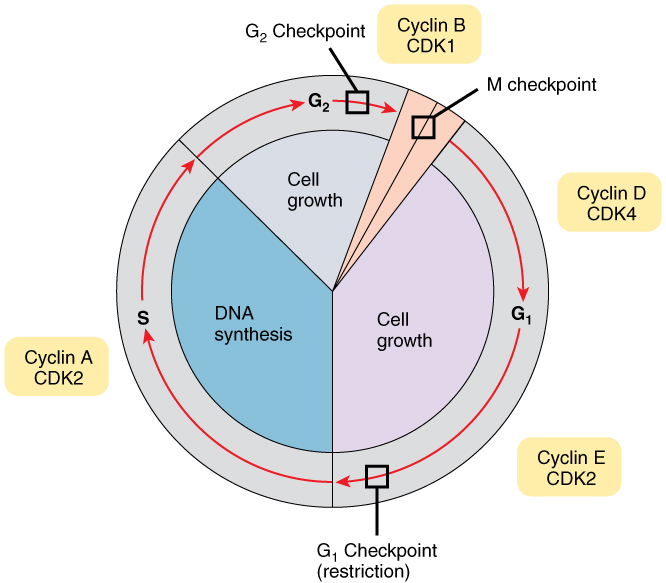
\includegraphics[width=0.5\textwidth]{Cell_Cycle}
	\caption{Representación del ciclo celular.}
	\label{fig:ciclo celular}
\end{figure}

Para nuestro modelo estableceremos que la célula pasa el \textit{punto de restricción}\footnote{El punto de restricción es el punto entre las fases $G_{1}$ y $S$, donde pasamos del crecimiento celular a la división (o apoptosis).} (ver Figura \ref{fig:ciclo celular}) si la concentración de Bcl-2 o de Rb de su entorno cae por debajo de cierto límite. Esto es, cuando el número de moléculas de Rb activas disminuye hasta un valor crítico, la célula abandona $G_1$ para iniciar la división celular y, cuando la cantidad de moléculas de Bcl-2 alcanza un umbral, la célula abandona $G_1$ para poner en marcha los mecanismos que llevan a la muerte celular. La variación temporal  de las concentraciones de Rb y Bcl-2 permite explicar la variabilidad observada en la duración de la fase $G_{1}$ de las células y, consecuentemente, en la duración de sus vidas.

\subsection{Los receptores de membrana regulan las dinámicas de Rb y Bcl-2}
\label{sub:hip_recep}

La fluctuación en la cantidad de Rb y Bcl-2 depende de unas proteínas llamadas \textit{citoquinas}, que ya fueron mencionadas en la Sección \ref{sec:cuestInmuno}. Estas pueden inducir tanto la fosforilación de Rb, en cuyo caso se denominan \textit{citoquinas de proliferación}, como tener un efecto positivo o negativo en cuanto a la cantidad de Bcl-2 se refiere, en ese caso nos referiremos a ellas como \textit{citoquinas de supervivencia} o \textit{muerte}, respectivamente.

La acción que las \textit{citoquinas} llevan a cabo se produce gracias sus interacciones con receptores de membrana específicos. De esta manera, el efecto que percibe una célula T depende, no solo de la cantidad de \textit{citoquinas} del ambiente, sino también del número de receptores de membrana de la célula. Si, por ejemplo, tenemos una concentración muy alta de cierta \textit{citoquina}, podríamos asumir que el efecto que esta va a tener en una célula T vendrá determinado por la cantidad de receptores de membrana específicos para ella que posea la célula en cuestión. También sabemos que el número de receptores de membrana de una célula varía a lo largo de su vida, haciendo así que células adyacentes que compartan un entorno similar (en el que la concentración de \textit{citoquinas} sea la misma, por ejemplo) presenten comportamientos distintos si expresan diferentes receptores de membrana.

\subsection{Las células T \textit{naïve} se dividen de manera asimétrica después de su activación.}
\label{sub:hip_divAsim}

Postulamos que tanto los fenotipos de las células T efectoras como los de las células T con memoria se determinan durante la sinapsis inmune. Esto es, una célula T en estado \textit{naïve} puede diferenciarse en una célula T efectora o en una célula T de memoria. Por su parte, tras esta primera división, las células T efectoras y de memoria, se dividen de manera simétrica, es decir, las células hijas heredarán el tipo de la madre, y ambos tipos se comportan de forma similar durante la respuesta inmune.

\section{Modelo matemático}
\label{sec:modelo}

Basándonos en las hipótesis anteriormente formuladas proponemos a continuación una serie de ecuaciones, con variables continuas y discretas, que darán forma al algoritmo de decisión de nuestro estudio. Como ya habíamos avanzado, se trata de un modelo simple, en el que los sistemas de ecuaciones diferenciales de primer orden propuestos tienen solución explícita. Sin embargo, es esta simplicidad la que hace de él un modelo tan potente, pues, como veremos en el capítulo siguiente, obtendremos resultados que no solo se ajustan a los hechos observados, sino que sacan a la luz comportamientos poblacionales difícilmente observables desde un laboratorio.

Antes de expresar en términos matemáticos las condiciones del modelo, estableceremos la notación a seguir y haremos algunas aclaraciones previas: 

\begin{itemize}
	\item Denotaremos por \textit{$c(t)$} y \textit{$a(t)$} la cantidad de Rb y Bcl-2 activa en tiempo $t$, respectivamente.

	\item Establecemos, sin pérdida de generalidad, que los límites que determinan la decisión entre división o apoptosis (ver hipótesis \ref{subsec:hip_1}) estarán en $c(t)=0$ y $a(t)=0$, respectivamente. De acuerdo a esta hipótesis definimos: 
	
	\begin{itemize}
		\item \textit{Decisión}: Fase que parte desde el nacimiento de la célula hasta que una de las células inhibidoras alcanza el límite establecido.
		
		\item \textit{Ciclo}: Fase que se extiende desde la \textit{punto de restricción} hasta la división celular.
		
		\item \textit{Apoptosis}: Tiempo de vida de la célula que comprende desde la desactivación de Bcl-2 y la finalización del programa de muerte celular ACAD (\textit{Activated T Cell Autonomous Death}).
		
		\item \textit{División}: Estado final después de que la célula haya entrado en la fase de ciclo.
		
		\item \textit{Muerte}: Estado final después de haberse completado la fase de apoptosis.
	\end{itemize}

	\item \textit{$R_{i}$} será el receptor de la i-ésima citoquina y \textit{$r_{i}(t)$} será la cantidad de ese receptor en tiempo $t$. 
	\item $r_{T}$ es el número de señales TCR/antíeno percibidas por la célula T correspondiente.
	
	\item Los parámetros $\mu_{Tc}$ y $\mu_{Ta}$ denotan la tasa de cambio de las moléculas inhibidoras por cada señal del TCR. A su vez los parámetros $\mu_{ic}$ y $\mu_{ia}$ representan la tasas de cambio de las moléculas inhibidoras por cada señal $R_i$.
	
	\item $\lambda_{Tj}$ es la tasa de cambio del receptor $R_{j}$ por cada señal del TCR. Por su parte $\lambda_{ij}$ es la tasa de cambio del receptor $R_j$ por cada señal $R_i$.
	
	\item $k$ es el número de receptores de membrana.
\end{itemize} 

Así las cosas, ya estamos en condiciones de presentar las ecuaciones del modelo. Como ya hemos visto en la Sección \ref{sec:hip_bio}, la dinámica de los inhibidores está controlada por las señales que recibe la célula de sus receptores de membrana durante la fase de decisión. Además, este número de señales depende del número de receptores de la célula. De acuerdo con estas observaciones, proponemos las siguientes ecuaciones:

\begin{equation}
	\label{sist_inhib}
	\left\{ \begin{array}{l}
	\dot{c}(t) = \mu_{Tc}r_{T}(t) + \sum_{j=1}^{k}\mu_{jc}r_{j}(t)\\
	\dot{a}(t) = \mu_{Ta}r_{T}(t) + \sum_{j=1}^{k}\mu_{ja}r_{j}(t) \\
	\end{array}
	\right.
\end{equation}

Con el Sistema \ref{sist_inhib}, ponemos de manifiesto que las concentraciones de Rb y Bcl-2, representadas por $c(t)$ y $a(t)$, respectivamente, dependen del número de señales TCR/antígeno ($r_{T}$) y, del número de receptores de membrana que posea la célula en cuestión.

Asumimos que los receptores de membrana involucrados en el algoritmo de decisión de las células T son independientes y tienen efectos aditivos. Según la hipótesis \ref{sub:hip_recep}, asumimos que las células son capaces de ``contar'' el número de señales que llegan. De acuerdo con estas relaciones lineales obtenemos un modelo robusto, puesto que configuraciones similares de receptores de membrana provocarán decisiones celulares similares. Teniendo en cuenta lo anterior proponemos la siguiente ecuación para los receptores de membrana:



\begin{equation}
	\label{sist_recep}
	\begin{array}{ll}
	\dot{r}_{i}(t) = \lambda_{Ti}r_{T}(t) + \sum_{j=1}^{k}\lambda_{ji}r_{j}(t) & \mbox{para $i=1,...,k$} 
	\end{array}
\end{equation}


\subsubsection{Aspectos técnicos del modelo}

En esta breve sección presentamos algunos aspectos técnicos del algoritmo propuesto, entre los que se incluyen las condiciones que marcaran en cambio de fase de una célula T, es decir, la condición que propiciará el paso de la fase de \textit{decisión} a \textit{ciclo}, por ejemplo, o los parámetros asignados a las células hijas al nacer .

\begin{itemize}
	\item Las condiciones $a(t)\geq0$, $c(t)\geq0$ y $r_i(t)\geq0$, para $i=1,...,k$ definen el domino de las ecuaciones \ref{sist_inhib} y \ref{sist_recep} durante la fase de decisión. 
	
	\item Cualquier receptor con valor negarivo $r_i(t)\leq0$ es \textit{reseteado} a 0 sin cambiar la fase de decisión en la que está la célula.
	
	\item Por su parte, las condiciones $a(t)=0$, $c(t)=0$ desencadenan el inicio de la fase de apoptosis y ciclo, respectivamente. Estas fases son excluyentes y no se pueden revertir mediante estimulación por \textit{citoquinas}. Además, tienen longitud constante que denotaremos por $t_{apo}$ y $t_{cycle}$.
	
	\item Si la célula progresa en la fase de ciclo los valores de $a(t)$ y $c(t)$ deben ser reiniciados para que las células hijas puedan comenzar la fase de decisión otra vez. 
	
	\item Una vez que la célula termina la fase de apoptosis es retirada de la población.
	
	\item Los parámetros $\lambda_{ji}$, $\mu_{ic}$, $\mu_{ia}$, $\mu_{Tc}$, $\mu_{Ta}$, $c(0)$ y $a(0)$ se consideran parámetros estructurales, es decir, se refieren a procesos biológicos que permanecen constantes durante la simulación. Por su parte, los parámetros referentes a la composición de receptores de membrana para una célula concreta $r_{i0}$ dependen de la historia de encuentros con el antígeno que ha tenido su madre y diferirán entre las células hijas cuando esta se divida (veremos cómo en la sección siguiente).
\end{itemize}


\section{Dinámica del \textit{patógeno} durante la respuesta inmune}
\label{sec:modeloPatCelT}

Ahora que ya tenemos un algoritmo para la dinámica de población de las células T, modelizamos la interacción del \textit{patógeno} con estas células. Debemos recordar que la dinámica de un \textit{patógeno} depende en gran cantidad de las características de este. Sin embargo, en esta sección daremos unas ecuaciones muy generales para que sean aplicables a la mayor cantidad posible de situaciones. En concreto, la dinámica del \textit{patógeno} vendrá dada por:

\begin{equation}
	\label{sist_pat_T}
	\begin{array}{ll}
	\dot{y}(t) = \alpha y(t) - \beta n(t)y(t)
	\end{array}
\end{equation} 

Donde $y(t)$ y $n(t)$ denotan el número de células del \textit{patógeno} y el número de células T, respectivamente. Los parámetros $\alpha$ y $\beta$ son positivos y dependen del antígeno: $\alpha$ representa la tasa de proliferación del \textit{patógeno}, mientras que $\beta$ corresponde a la tasa de eliminación del mismo a causa de las células T.

De acuerdo con este modelo, podemos ver que el \textit{patógeno} aumenta su población hasta que el número de células T alcanza cierto valor, en ese momento $\dot{y}(t)$ se hace negativa y, en consecuencia, $y(t)$ comienza a decrecer. Asumiremos que las señales captadas por el TCR de una célula T son proporcionales al número de encuentros que tenga con el antígeno. Si llamamos al número de señales TCR de una célula $x$ en tiempo $t$, $r_{T}^{x}(t)$, tenemos:

\begin{equation}
	\label{ec:rhotau}
	r_{T}^{x}(t) = \gamma\rho_{n}^{x}y(t)
\end{equation}

Donde $\gamma$ es un parámetro que depende del antígeno y denota la probabilidad de que haya una activación del TCR debido a un encuentro con el antígeno. Por otro lado, $\rho_{n}^{x}$ representa la cantidad de antígeno que está disponible para una célula T, $x$, en porcentaje. Luego:

\begin{equation}
	\sum_{x=1}^{n} \rho_{n}^{x} \leq 1
\end{equation}

Según la hipótesis \ref{sub:hip_divAsim}, las células T que ya se han diferenciado se dividen de manera simétrica y reparten sus receptores de membrana entre sus dos células hijas. De esta manera, la experiencia con el antígeno, propia de cada célula puede ser transmitida a la siguiente generación.

\begin{equation}
	\label{sist:div_sim}
	\left\{ \begin{array}{l}
	r_{i0}^{1}= \delta_{i}^{x} r_{i}^{x}\\
	r_{i0}^{2}= (1-\delta_{i}^{x}) r_{i}^{x} \\
	\end{array}
	\right.
\end{equation}


Donde $\delta_{i}^{x}$ representa el ratio de receptores de membrana de tipo $R_{i}$ entre las células hijas, $r_{i0}^{1}$ y $r_{i0}^{2}$ denotan los valores iniciales de receptor $R_{i}$ en las células hijas 1 y 2, respectivamente, y  $r_{i}^{x}$ denota el número de receptores $R_{i}$ en la célula T $x$ en el momento de la división celular.


Ahora que hemos descrito los conceptos matemáticos que representan las hipótesis biológicas que sustentan este modelo, estamos en condiciones de estudiar las soluciones de las ecuaciones correspondientes y de interpretar en términos biológicos los resultados obtenidos. En el capítulo siguiente presentaremos simulaciones numéricas de este mismo modelo en un caso simplificado, en el que se supone que el número de receptores de membrana es dos ($k = 2$). En ese capítulo se discutirán diferentes situaciones: tolerancia e intolerancia al \textit{patógeno} o respuesta inmune en el caso de poblaciones de células T con distintas afinidades al \textit{patógeno}. Todas estas situaciones han sido reproducidas a partir del mismo modelo, con el simple cambio del valor de sus parámetros, poniendo de manifiesto la capacidad del mismo para reproducir con facilidad situaciones diversas. 

%\section{Resumen y conclusiones}

%Antes de embarcarnos en las simulaciones de este modelo, vamos a resumir los aspectos más importantes de este capítulo con la finalidad de que el capítulo siguiente resulte más cómodo de leer.
%
%Lista de puntos clave:

%\begin{enumerate}
%	\item El algoritmo determina qué decisión, división o suicidio, toman las células T.
%	\item Las decisiones se toman de manera individual y se basan en la información que reciben del entorno a través de su TCR.
%	\item Lo que decide qué decisión se toma y cuándo es la cantidad de ciertas moléculas inhibidoras.
%	\item Ciclo y apoptosis son fases mutuamente exclusivas e irreversibles.
%	\item Cuando una célula T se divide sus hijas son del mismo tipo y comparten sus receptores de membrana.
%	\item Cuando una célula muere se elimina de la población.
%	\item El crecimiento del antígeno depende del número de células T y decrece cuando las células T comienzan a crecer.
%	\item Cuando las células T detectan al patógeno su población crece rápidamente y decrece también rápidamente cuando el patógeno ha sido vencido, aunque con cierto desfase.
%	\item En la última etapa de la respuesta inmune coexisten dos tipos de linfocitos T: los linfocitos sensibles a la apoptosis, que mueren durante la \textit{contracción clonal} (efectores), los linfocitos resistentes a la apoptosis, que	sobreviven en forma de linfocitos de memoria.
%\end{enumerate} 




